

\documentclass[a4paper,11pt]{article} 
\usepackage[spanish]{babel}           
\usepackage[utf8]{inputenc}           

\usepackage[T1]{fontenc}   		   % Fonte por defecto.
\usepackage{graphicx, subfigure}    		   % Engadir imaxes.
\usepackage{color}      		   % Uso de cores.
\usepackage{anysize}     		   % Modificar o tamaño dos marxes.
\usepackage{multicol, multirow}    % Escribir a doble, triple...columna.
\usepackage{bm}          		   % Letras gregas en negriña.
\usepackage{textcomp}    		   % Símbolos, poden consultarse na rede.
\usepackage{eurosym}     		   % Símbolo € (\euro).
\usepackage{amsthm}                % Paquete da AMS para escribir teoremas.
\usepackage{amsmath,amsfonts}      %Paquetes específicos de símbolos.
\usepackage{lineno}                % Numerar as liñas. 

\marginsize{1.5cm}{1.5cm}{1.5cm}{1.5cm} % MARXES: Esq, der, sup, inf.
\parindent=0mm                        % Sangría. 
\parskip=2mm                          % Espazo entre párrafos.
\renewcommand{\baselinestretch}{1}    % Interliñado.
\renewcommand{\spanishtablename}{Táboa} 


\title{Tema 2: Memoria a curto prazo e memoria de traballo}
\date{}


\begin{document}  

\maketitle 

\section{Memoria a curto prazo versus memoria de traballo}
Existen diferentes etiquetas para referirse ó mesmo compoñente da memoria: memoria primaria, elemental, inmediata, MCP, temporal, de traballo, operativa... Este é o primeiro sistema de memoria do que somos conscientes. Porén, non é o mesmo que a consciencia: somos conscientes dos contidos da MCP, pero non temos por que selo dos seus procesos. 

Estas dúas memorias teñen connotacións diferentes:
\begin{itemize}
	\item \textbf{Memoria a curto prazo (MCP):} É máis antiga. Fai referencia ó almacenamento de
	pequenas porcións de información durante un breve intervalo temporal. Os sistemas responsables da 
	MCP forman parte do sistema de memoria de traballo.  
	\item \textbf{Memoria de traballo ou operativa:} Refírese a un espacio de traballo mental 				temporal, no que se mantén e se manipula a información ó mesmo tempo, permitindo o 						desenvolvemento de actividades cognitivas complexas como razoar, comprender e aprender.
\end{itemize}

O termo <<MCP>> fai referencia a unha situación experimental. O termo <<memoria de traballo>> baséase nun suposto teórico segundo o cal tarefas como razoar ou aprender dependerían dun sistema capaz de manter e manipular a información temporalmente. Este sistema constituiría un espacio mental.

\section{Capacidade da memoria a curto prazo}
Mídese habitualmente co ``Test de amplitude de díxitos'', que consiste en memorizar unha lista de valores de 4 a 10 unidades. Os resultados habituais sitúanse entre as 5 e as 7 unidades de información. 

A amplitude da memoria inmediata é o maior número de ítems que poden lembrarse na orde correcta, inmediatamente despois da súa presentación. Para levar a cabo tarefas de amplitude deben lembrarse os \textit{ítems} presentados así como a \textit{orde} de presentación dos mesmos. 

Memorizar os ítems é relativamente sinxelo se os coñecemos e comprendemos. A orde lémbrase grazas ó proceso de encadeamento, que consiste en asociar un ítem ó seguinte sucesivamente. Porén, se se olvida un ítem da cadea, os seguintes son máis difíciles de lembrar. 

George Miller (1956) suxire que a amplitude de memoria non se limita a un número de ítems, senon a un número de \textit{chunks}, grupos de información subxectivos e organizados nun patrón familiar. 

O \textit{chunking}, ou formación de grupos, consiste en agrupar unha serie de ítems aleatorios nun número menor de elementos significativos para mellorar o recordo. Pode darse grazas á consistencia dos ítems cos hábitos lingüísticos, á entoación coa que se pronuncian, ás pausas entre eles, etc.

Conrad e Hull (1964) demostran que a memoria para secuencias de consoantes é sustancialmente máis pobre cando estas teñen unha sonoridade parecida. Interpretan os seus resultados en termos dun almacén de memoria a curto prazo que se apoia nun código acústico, que desaparece con rapidez, producindo o olvido. Así, como as letras acusticamente semellantes posúen menos características distintivas, cada ítem confúndese co adxacente e aparecen erros na orde de recuperación.

\section{Duración da memoria a curto prazo e olvido}
Peterson e Peterson (1959) deseñan unha experiencia de olvido na que proporcionan ós suxeitos un ítem a recordar (un conxunto de tres consoantes), para logo distraelos pedíndolles que contasen ó revés de tres en tres a partir dun número dado. Despois duns segundos contando, pedíanlles que lembrasen o ítem. 

\begin{figure}[h!]
	\centering
	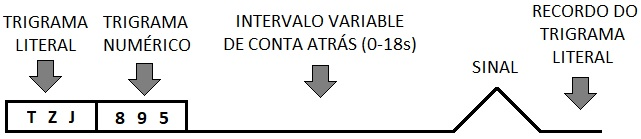
\includegraphics[width=0.55\linewidth]{memoria2_1}
	\caption{Exemplo dun ensaio na tarefa de Peterson}
\end{figure}

Os Peterson suxiren que os resultados reflexan o decaemento rápido dunha pegada de memoria a curto prazo, o que concorda coas conclusións de Brown do olvido a curto prazo. O olvido a longo prazo explicaríase por interferencia. 

Máis adiante cuestiónanse estas reflexións e atópanse dúas posibles fontes de interferencia na tarefa:
\begin{itemize}
	\item[-] A tarefa distractora que impide o repaso.
	\item[-] A causada polos trigramas anteriores, que se parecen ós ítems a recordar. Así, cada
	ensaio (menos o primeiro) sofre a interferencia dos precedentes (interferencia proactiva).
\end{itemize}

A solución ó debate interferencia-decaemento ven dada pola proposta de Reitman (1971-1974): a memoria está determinada pola forza da pegada, que decae co paso do tempo, e pola cantidade de interferencia presente. É semellante á detección dun sinal (información a recordar) nun fondo ruidoso (interferencia). 

\section{Recuperación na memoria a curto prazo}
\subsection{O modelo de búsqueda serial de Stenberg}
Stenberg supón que se activa temporalmente a información almacenada na MCP para evocala. Interésalle saber como se recupera esta información. Para averigualo deseña tarefas de recoñecemento de alta precisión, nas que emprega o tempo de reacción (TR) como principal VD. 

A <<Tarefa de recoñecemento de ítems>> comeza coa memorización dunha lista de elementos (números ou palabras). Logo pregúntaselle ó suxeito acerca dun elemento concreto, que pode estar ou non na lista, e mídese o tempo que tarda en responder. Este proceso repítese ó longo de varios ensaios.

\begin{figure}[h!]
	\centering
	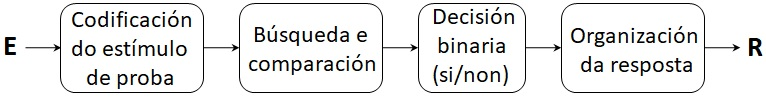
\includegraphics[width=0.58\linewidth]{memoria2_2}
	\caption{Modelo de procesos mentais que interveñen na tarefa}
\end{figure}

Plantéxanse dúas cuestións acerca do proceso de búsqueda:
\begin{enumerate}
	\item Decidir entre dous modelos alternativos de búsqueda (``serial'' ou ``en paralelo'').
	Fanse prediccións empíricas sobre o efecto do tamaño do conxunto de memoria. Os resultados apoian
	a búsqueda serial.
	\item Decidir entre dous modelos alternativos de búsqueda serial (``autoterminada'' ou
	``exhaustiva''). De novo, fanse prediccións empíricas sobre o efecto do tamaño do conxunto de 			memoria, e sobre os efectos de exposición serial. Os resultados apoian a búsqueda exhaustiva.
\end{enumerate}

Intuitivamente parece máis lóxico supoñer que o proceso de comparación debería deterse unha vez se atopa o ítem nos casos positivos, o que constituiría unha búsqueda autoterminada. Porén, Sternberg considera que a búsqueda exhaustiva é máis eficiente ó entender a comparación e a decisión como procesos mentais separados, e sabendo que as decisións adoitan consumir máis tempo que as comparacións.

\subsection{Avaliación crítica do modelo de Stenberg}
O modelo deixa varios fenómenos experimentais sen explicar: a variabilidade dos TR, o efecto da semellanza entre o ítem de proba e os do conxunto de memoria e o axuste precisión-velocidade. Tamén se lle critica a interpretación alternativa respecto ó incremento do TR en función do tamaño do conxunto de memoria e as etapas de procesamento secuenciais e independentes. 

Con todo, o traballo de Sternberg un gran avance na investigación cronométrica, e o seu modelo segue empregándose sobre todo en contextos aplicados. Por este motivo coñécese que as medidas independentes obtidas da tarefa (pendiente da función e valor de intersección) parecen ser sensibles ós efectos de drogas e dano cerebral. 

A tarefa adoita incluirse tamén en probas de intelixencia. 

\subsection{Curva de posición serial: resultados do paradigma de recordo libre}
A probabilidade de recordo dun ítem determinado diminúe a medida que aumente a lonxitude da lista. Porén, o número absoluto de elementos lembrados aumenta coa lonxitude. Obsérvanse dous efectos:
\begin{itemize}
	\item \textbf{Efecto de primacía:} Tendencia a lembrar mellor os primeiros ítems dunha lista.
	Este efecto depende principalmente da MLP, e probablemente se relacione coa tendencia a repasar
	os primeiros ítems desde a súa presentación e ata o final da lista de estudo (porque é máis
	probable que entren na MLP e se lembren despois).
	\item \textbf{Efecto de recencia:} Tendencia a lembrar mellor os últimos ítems dunha lista,
	especialmente se o recordo é inmedianto. Este efecto elimínase cunha breve demora, ocupada por
	unha tarefa distractora.
\end{itemize}

Existen unha serie de factores que inflúen na MLP, así como na execución relativa ó recordo das porcións inicial e media das listas de estudo. O efecto de recencia e practicamente inmune a eles.
\begin{itemize}
	\item \underline{Tasa de presentación}: Unha presentación máis lenta mellora o recordo.
	\item \underline{Frecuencia das palabras}: As palabras familiares recórdanse mellor.
	\item \underline{Imaxinabilidade}: As palabras máis visualizables son máis sinxelas de lembrar.
	\item \underline{Idade}: Os adultos xóvenes recordan mellor que os nenos ou os ancianos.
	\item \underline{Estado fisiolóxico}: As drogas (alcohol, mariguana) perxudican o rendemento.
\end{itemize}

\subsubsection{Efecto de recencia}
Inicialmente pénsase que a recencia, a diferencia da primacía, reflexa a resposta dun almacén temporal a curto prazo. Obsérvase que a realización dunha tarefa distractora despois da lista de estudo interrumpe este almacenamento a curto prazo e elimina a recencia.

Porén, atópase que a presentación de dita tarefa distractora despois de cada ítem da lista provoca un novo efecto de recencia. Estes efectos danse incluso con intervalos extremos, coma meses, o que fai imposible que os ítems se manteñan no almacén a curto prazo. Así descóbrese o efecto de recencia a longo prazo. 

O efecto de recencia reflexa unha estratexia de recuperación particular: os eventos máis recentes son os máis facilmente dispoñibles para lembrar en función dunha razón de discriminación, baseada na distancia temporal entre o ítem a recuperar e o seu competidor máis próximo.

Isto explícase ben coa \textit{metáfora do poste telefónico} de Crowder (1974). O poste que mellor observamos é o que está máis preto de nós. Ó aumentar a distancia, aumenta tamén a dificultade para distinguir un poste doutro. No caso dos ítems, o máis recente recórdase e distínguese perfectamente dos demais, pero as demoras crecentes fan que a fan que diminúa progresivamente a capacidade de discriminar o resto de ítems.

\section{Aproximacións neuropsicolóxicas ó estudo da memoria a curto prazo}
O paciente HM padece epilepsia non tratable. É operado para reducir os seus ataques, pero durante a intervención cáusanlle lesións quirúrxicas en ambos lados do cerebro, na rexión do hipocampo, estrutura fundamental na memoria episódica a longo prazo. Os seus ataques diminúen, pero queda afectado de amnesia densa. 

HM ve deteriorada a súa capacidade para aprender material novo (visual e verbal) e non pode actualizar o seu coñecemento sobre o mundo, pero conserva algúns aspectos da súa memoria: pode lembrar eventos ocorridos antes da operación e aprender tarefas de tipo motor, e conserva a súa capacidade de amplitude de díxitos.

O estado do paciente suxire que a execución relativa á MCP e á MLP podería depender de sistemas de memoria diferentes, ligados a áreas cerebrais distintas. Así, iníciase un estudo consistente na observación de pacientes con amnesia densa que presentan un intelecto normal. Examínase a súa execución en varias tarefas de MCP e MLP, e os resultados son:
\begin{itemize}
	\item[•] Execución normal na tarefa de Peterson (MCP).
	\item[•] Capacidade de amplitude de díxitos (MCP).
	\item[•] Recencia intacta en recordo libre (MCP).
	\item[•] Capacidade de adquirir novas habilidades motoras (MLP implícita).
	\item[•] Déficit en primacía e outros ítems iniciais das listas de recordo libre (MLP explícita). 
	\item[•] Deterioro na adquisición de novas memorias episódicas e semánticas (MLP explícita).
\end{itemize} 

Por outra banda, outros pacientes como KF presentan serios deterioros en amplitude de díxitos, na tarefa de Peterson e na recencia en recordo libre. Así constitúense dous grupos de pacientes: o A, con execución normal en MCP e deterioro en MLP, e o B, co patrón contraria. Estes grupos representan a <<doble disociación>> neuropsicolóxica, unha proba sólida da existencia de, polo menos, dous sistemas ou procesos separados de memoria. 

Outro tipo de disociacións serían:
\begin{itemize}
	\item Os pacientes como KF e PV, cun déficit específico do compoñente fonolóxico da MCP. A súa
	amplitude de díxitos, normalmente de dous, aumenta cando se pon a proba mediante a presentación 		visual. Presentan unha reducción drástica do efecto de recencia no recordo libre inmediato de 			tipo verbal, pero a súa recencia a longo prazo é normal. É dicir, son capaces de empregar unha
	estratexia de recencia, pero son incapaces de facelo para aumentar a memoria verbal inmediata
	(que se basea nun código fonolóxico ou verbal/léxico).
	\item Os pacientes como MV, LH e LE, cun déficit específico na MCP visual e espacial, pero con 			MCP verbal normal. LH ten dificultades para recoñecer formas e cores, pero posúe unha memoria 			espacial excelente. LE posúe memoria espacial pero a súa memoria visual está deteriorada (é
	escultora; tras a lesión, o seu estilo vólvese abstracto e os seus debuxos menos realistas). Por
	último, MV posúe memoria visual normal, pero as súas capacidades espaciais están deterioradas. 
\end{itemize}

\section{O modelo multicompoñente da memoria de traballo}
\subsection{Problemas co modelo modal de Atkinson e Shiffrin}
Como xa vimos, o modelo modal asume que a información entra do ambiente e é procesada por unha serie de sistemas de memoria sensorial de curta duración. Logo flúe cara o almacén a curto prazo, que se encarga de pasar a información cara e desde o almacén a longo prazo, e que ademais actúa como memoria de traballo. Esta memoria é responsable de activar estratexias, do repaso e constitúe un espazo global de traballo. 

Este modelo enfróntase rapidamente a dous problemas:
\begin{enumerate}
	\item Supón que o mantemento de ítems na memoria a curto prazo garantiza a aprendizaxe a longo
	prazo. Isto cuestiónano Craik e Lockhart (1972) e propoñen o principio dos <<niveis de
	procesamento>>, que di que a aprendizaxe depende da maneira en que se procesa o material, máis
	ca do tempo que pasa na MCP.
	\item Segundo o modelo, un déficit de MCP ocasionaría graves problemas de aprendizaxe a longo
	prazo e dificultades para levar a cabo actividades cognitivas complexas (razoar e comprender).
	Porén, moitos estudos neuropsicolóxicos sobre pacientes con deterioros en MCP amosan que estos
	non sofren un déficit xeral na súa MLP ou na memoria de traballo.
\end{enumerate}

\subsection{A técnica da tarefa secundaria ou dual (Baddeley e Hitch, 1974)}
A tarefa dual aparece nunha investigación sobre a relación entre a MCP e a MLP, na que se busca a función do sistema ou sistemas subxacentes á MCP. Baddeley e Hitch reclutan unha mostra de estudantes de grao e combinan dúas tarefas ó mesmo tempo: unha de amplitude de díxitos e outra de razoamento, comprensión e aprendizaxe.

Piden ós participantes que repasen continuamente e en voz alta unha secuencia de díxitos (de 0 a 8), ó mesmo tempo que realizan unha tarefa cognitiva (razoamento verbal). Suponse que ambas tarefas están controladas pola MCP, cuxa capacidade é limitada. Así, canto máis longa sexa a secuencia de díxitos maior será a interferencia coa tarefa principal. 

O resultado é que os participantes son quen de levar a cabo a tarefa cognitiva, cunha tasa de erro constante do 5\%. O tempo medio para a verificación das frases aumenta coa carga de díxitos, pero non de xeito abrumador.

\newpage

\begin{figure}[h!]
	\centering
	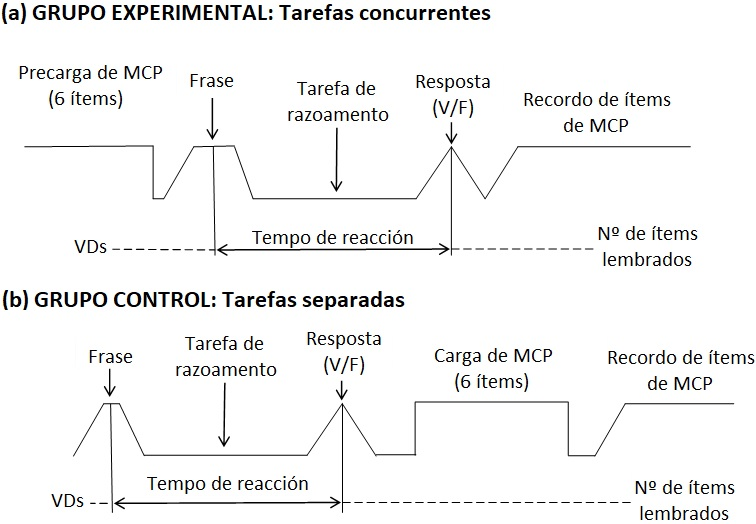
\includegraphics[width=0.6\linewidth]{memoria2_3}
	\caption{Secuencia de tarefas en ensaios experimental e de control}
\end{figure}

Segundo os autores, a MCP é un compoñente dun sistema máis complexo, a memoria de traballo. Así, a tarefa de razoamento depende da capacidade xeral (e limitada) da MT. O mantemento dun ou dous ítems, que non perturba a MT, depende probablemente dun compoñente específico (bucle fonolóxico). Este bucle podería sobrecargarse co mantemento de 6 ou máis ítems, e nese caso, empregaría os recursos mentais do compoñente xeral de MT.

\subsection{O modelo multicompoñente da MT}
\begin{figure}[h!]
	\centering
	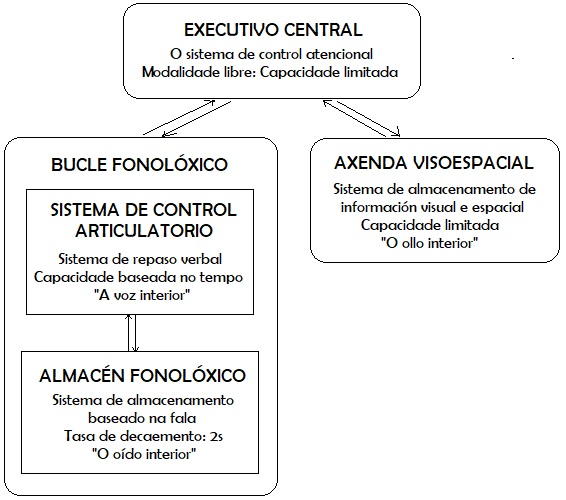
\includegraphics[width=0.6\linewidth]{memoria2_4}
	\caption{Representación simplificada do modelo de memoria de traballo de Baddeley (1990)}
\end{figure}

\begin{itemize}
	\item \textbf{Executivo central:} Sistema atencional de capacidade limitada que selecciona e
	manipula material nos subsistemas, actuando como un controlador que xestiona a actividade.
	\begin{itemize}
		\item \underline{Bucle fonolóxico}: Especializado en manter secuencias de elementos acústicos
		e relacionados coa fala.
		\begin{itemize}
			\item \textbf{Almacén fonolóxico:} Mantén a información entre 1,5 e 2 segundos.
			\item \textbf{Sistema de control articulatorio:} Realiza dúas funcións:
			\begin{itemize}
				\item Mantén a información verbal dentro do almacén fonolóxico mediante un repaso
				subvocal (refrescando as pegadas de memoria antes de que desaparezan).
				\item Manexa material verbal presentado visualmente e rexístrao no almacén
				fonolóxico, mediante a subvocalización (convertíndoo a un código fonolóxico).
			\end{itemize}
		\end{itemize}
		\item \underline{Axenda visoespacial}: Realiza unha función semellante á do bucle, pero con
		elementos e secuencias codificadas visual e/ou espacialmente. 
	\end{itemize}
\end{itemize}

\subsubsection{Blucle fonolóxico}
Presentamos a continuación unha serie de datos empíricos que apoian a existencia do bucle fonolóxico:
\begin{itemize}
	\item \underline{Efecto de similitude fonolóxica}: Tendencia a que os erros dos suxeitos sexan
	fonoloxicamente semellantes ó ítem correcto, e deterioro no recordo serial inmediato de destes
	ítems. Isto non ocorre, por exemplo, coa semellanza de significado, porque o almacén baséase nun
	código fonolóxico.
	\item \underline{Efecto da fala irrelevante ou non atendida}: Reducción no recordo serial
	inmediato de listas de ítems presentados visualmente debido á presenza de material falado
	irrelevante. Isto ocorre porque o material falado, aínda que irrelevante, ten acceso directo ó
	material fonolóxico.
	\item \underline{Efecto de lonxitude das palabras}: A amplitude de memoria é inversamente
	proporcional á lonxitude das palabras. Este efecto depende da duración da articulación das
	palabras, o que indica que a limitación do bucle fonolóxico é temporal.
	\item \underline{Efecto de supresión articulatoria}: Cando se impide que os suxeitos realicen un
	repaso subvocal, pedíndolles que repitan un ítem irrelevante, a amplitude de memoria inmediata
	redúcese significativamente (independentemente de que a presentación do material sexa auditiva ou
	visual). Isto dase porque a articulación do ítem irrelevante domina o proceso de control
	articulatorio, impedindo o seu uso.
\end{itemize}

Na cognición cotiá, o bucle é importante para aprender a ler, adquirir vocabulario e comprender a linguaxe. Sabémolo grazas a estudos sobre o desenvolvemento da linguaxe en nenos normais e sobre o rendemento de pacientes con déficit en MCP debido a danos cerebrais. 

En 1990, Gathercole e Baddeley investigan se o bucle fonolóxico inflúe na adquisición da lingua materna. Avalían a un grupo de nenos de 8 anos cun déficit lingüístico específico. A intelixencia non verbal destes nenos é normal, pero o seu desenvolvemento lingüístico corresponde a nenos de 6 anos.

Preséntanlles unha batería de tests de memoria, e observan que teñen dificultades para repetir pseudopalabras non familiares. Así, desenvolven un ``Test de repetición de pseudopalabras'', no que os nenos escoitan pseudopalabras de lonxitude cada vez máis extensa que teñen que repetir. Pasan o test a estes nenos, a nenos da mesma idade cun desenvolvemento lingüístico normal e a nenos de 6 anos, cuxo nivel de desenvolvemento lingüístico é equivalente ós do déficit pero cun nivel de execución non verbal menor, por seren máis pequenos. 

Os resultados mostran que a execución dos nenos de 8 anos con trastorno lingüístico é aínda menor que a dos de 6 anos. A súa capacidade de repetición de pseudopalabras é equivalente á de nenos de 4 anos.

Investigacións posteriores demostran que a memoria fonolóxica é o factor crucial na fase de adquisición de vocabulario. Porén, conforme os nenos medran, aumenta a súa capacidade para empregar vocabulario xa coñecido para aprender novas palabras.

\subsubsection{Axenda visoespacial}
É a responsable da creación e manipulación de imaxes visuais. Pode alimentarse de forma directa, a través da percepción, ou indirecta, xerando unha imaxe visual. Parece estar implicada no uso de mnemotecnias baseadas en imaxes visuais. 

Hai evidencias da existencia de dous subcompoñentes neste sistema:
\begin{enumerate}
	\item Un compoñente visual relacionado co procesamento de patróns e coa detección do ``que''.
	\item Un compoñente espacial relacionado coa localización no espazo e coa información acerca do
	``onde''.
\end{enumerate}

É probable que este sistema espacial sexa importante para a orientación xeográfica e para planificar tarefas espaciais. Ademais, as tarefas de manipulación visoespacial adoitan ser un compoñente importante dos tests de intelixencia, empregándose frecuentemente como instrumentos de selección para enxeñaría e arquitectura. 

\subsubsection{Executivo central}
A MT está dirixida polo executivo central, un controlador atencional máis que un sistema de memoria. A súa forma de operar propóñena Norman e Shallice (1986), plantexando a existencia de dous modos de control:
\begin{itemize}
	\item Un modo automático, baseado nos hábitos existentes. Consiste nun conxunto de procedementos
	sobreaprendidos que permiten resolver conflitos automaticamente. Ó basearse en hábitos ben
	aprendidos, estes procedementos requiren pouca atención (\textit{exemplo:} conducir).
	\item Un modo dependente dun executivo atencionalmente limitado. Actívase cando a resolución
	automática non é posible ou cando surxe unha situación novidosa. Este modo denomínase <<sistema
	atencional superior>> (SAS), e encárgase de optar por unha das opcións posibles ou de activar
	estratexias para buscar solucións alternativas. O seu papel é crucial no funcionamento do
	executivo central.
\end{itemize}

Os investigadores seguen dúas liñas de interés durante a elaboración do modelo. Por unha banda estudan os lapsus nas accións, onde un fallo atencional produce consecuencias non previstas. Trátase de situacións nas que o SAS deixa de operar cando debería facelo.

Por outro lado realizan estudos sobre pacientes con dano no lóbulo frontal, nos que detectan tres características:
\begin{itemize}
	\item \textbf{Problemas de control atencional:} Refléxanse en condutas de perseveración, como a
	execución repetida do mesmo acto ou a comisión repetida do mesmo erro.
	\item \textbf{Condutas de utilización:} Os pacientes (\textit{exemplo:} RR) son incapaces de
	focalizar a atención, e responden a calqueira obxecto presente no ambiente. En ausencia de
	control por parte do SAS responden a calqueira sinal proporcionado polo entorno. Asúmese polo
	tanto que os lóbulos frontais son necesarios para o correcto funcionamento do SAS, e que se se
	danan, o control atencional da acción pode fallar.
	\item \textbf{Monitorización da conduta:} Os lóbulos frontais tamén controlan que a conduta sexa
	a apropiada. Se fallan poden desencadearse condutas estrafalarias ou de fabulación.
\end{itemize}

Unha das funcións máis importantes do executivo central é o foco atencional, a capacidade de dirixir a atención cara a tarefa en curso. 

Nun estudo, Robins \textit{et al.} (1996) comparan os efectos producidos no recordo de posicións de xadrez mediante unha tarefa atencional moi demandante na que os participantes teñen que xerar secuencias de números aleatorias. Avalían tanto a xogadores expertos como a outros con pouca experiencia.

Os resultados amosan diferenzas importantes na execución global entre os grupos, pero ambos presentan o mesmo patrón de interferencia. A supresión articulatoria non produce efectos, o que suxire que o bucle fonolóxico non intervén. A tarefa viso-espacial perxudica a execución, e a maior perturbación prodúcea a xeración aleatoria. Os resultados mantéñense cando se cambia a tarefa de recordo de posicións por unha de elección do seguinte mellor movemento, o que sinala a importancia do papel da axenda e do executivo central en tarefas de planificación e de recordo de posicións.

Outra función do executivo central é a de dividir a atención entre dúas ou máis tarefas, como falar por teléfono mentras se conduce. En xeral é posible, pero se se introduce información espacial, esta pode interferir co control na conducción. Máis importante aínda é o efecto da tarefa de falar sobre a capacidade de tomar decisións correctas respecto á conducción: pode fallar a capacidade de avaliación. Este acto é perigoso polo que o cerebro deixa de facer mentras falamos, non porque teñamos as mans ocupadas.

Algúns estudos sobre pacientes con Alzheimer demostran que para eles é especialmente difícil dividir a atención entre varias tarefas, aínda que sexan sinxelas. Porén, isto non se da con tarefas únicas, nin sequera cando son difíciles. Destes estudos conclúese que os pacientes poderían ser capaces de manter unha conversación cunha soa persoa, pero poderían perder o fío se participasen máis.

En conclusión, algúns aspectos do cambio son automáticos e outros requiren atención. Cando se dan os segundos entra en xogo o executivo central.

\subsubsection{\textit{Buffer} ou retén episódico}
Un problema importante do modelo de memoria de traballo de tres compoñentes é explicar como se relaciona coa MLP. É dicir, saber como logra a MT beneficiarse da MLP. Existen tres exemplos concretos que non explica o modelo:
\begin{itemize}
	\item[-] A amplitude de memoria para o recordo de palabras nunha frase é arredor e 15, mentres
	que no caso de palabras non relacionadas é de 5 ou 6. Isto explícase porque a orde das palabras
	nunha frase segue leis gramaticais e posúe un significado. Estes factores permiten o proceso de
	agrupamento ou \textit{chunking}, que deriva nun aumento da amplitude de memoria, e ambos
	dependen da MLP.
	\item[-] A amplitude de díxitos é de 7 ou máis, e tendo en conta que 2 ou 3 van ó bucle, onde se
	almacenan os restantes? E se se almacenan na MCP visual, como se combina esta coa fonolóxica?
	\item[-] En canto á viveza de imaxes, as imaxes baseadas na MLP (recordo dunha escea) non
	parecen depender moito nin do sistema viso-espacial nin do fonolóxico.	
\end{itemize}

Para solucionar estes problemas, Baddeley (2000) propón a existencia dun cuarto compoñente: o \textit{buffer} episódico, un sistema de almacenamento capaz de manter catro bloques de información (\textit{chunks})nun código multidimensional. 

Grazas á súa capacidade de manter distintas dimensións, o \textit{buffer} actúa como enlace entre os subsistemas da memoria de traballo e conéctaos coa información enviada pola MLP e o sistema perceptivo. A información do \textit{buffer} recupérase a través do acceso consciente a el, idea que permite relacionar a memoria de traballo coa conciencia: a experiencia consciente encárgase de unir os distintos fluxos de información procedentes dos sentidos e ``integralos'' para formar as esceas e obxectos percibidos. 

Inicialmente, o \textit{buffer} plantéase como un sistema activo, totalmente controlado polo executivo central e capaz de integrar conceptos previamente non relacionados para crear novas combinacións. Enténdese que os procesos executivos son necesarios para integrar as palabras dunha frase e formar bloques con significado, ou para integrar rasgos perceptivos (formas e cores) nos obxectos percibidos. Así, o bloqueo do executivo mediante unha tarefa concurrente demandante debería interferir coa integración, pero non é así. 

Por este motivo tómase a idea de \textit{buffer} como un sistema máis pasivo: unha pantalla na que se proxecta información procedente de distintas fontes pero cuxo proceso de integración ocorre fóra da pantalla.

O modelo actual de memoria de traballo é unha elaboración do modelo orixinal de tres compoñentes con dous cambios fundamentais:
\begin{enumerate}
	\item O suposto de que existe unha conexión entre a MLP e os subsistemas fonolóxico e
	viso-espacial, que permiten a adquisición da linguaxe e de información visual e espacial.
	\item A inclusión do \textit{buffer} episódico, ó que é posible acceder desde o executivo
	central, os subsistemas fonolóxico e viso-espacial e a MLP. O \textit{buffer} tamén explica como
	inflúen as emocións na MT.
\end{enumerate}

\begin{figure}[h!]
	\centering
	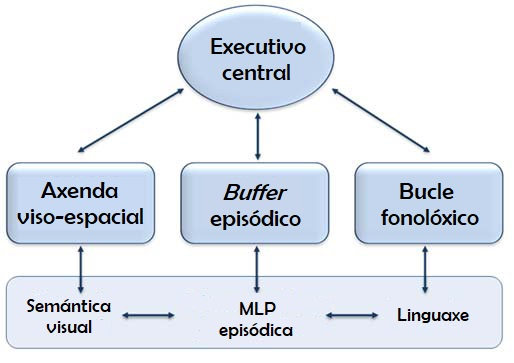
\includegraphics[width=0.4\linewidth]{memoria2_5}
	\caption{Modelo actual de MT}
\end{figure}

\section{Diferenzas individuais na memoria de traballo}
Daneman e Carpenter (1980) realizan un estudo sobre o posible papel da memoria de traballo na comprensión da linguaxe. Consideran como característica definitoria da MT a simultaneidade dos procesos de almacenamento e procesamento da información, e propóñense crear unha tarefa para medir este aspecto.

A tarefa resulta ser moi sinxela: consiste en ler unha secuencia de frases para logo repetir a última palabra de cada unha. Obtense que a amplitude de MT é de dúas a cinco frases.

Descóbrese que a amplitude nesta proba predí diversas capacidades, entre elas a comprensión de prosa, a mellor redacción, o seguimento de instruccións complexas e a realización de mellores apuntes. Ademais, existe unha correlación moi alta entre amplitude de MT e CI e entre amplitude de MT e intelixencia fluída.

Noutro estudo, Engle e Turner (1989) desenvolven unha tarefa consistente en lembrar palabras, cada unha das cales vai seguida por unha operación aritmética que hai que resolver. Obteñen así unha medida de amplitude operacional, que correlaciona altamente coa tarefa de amplitude de frases orixinal.

As persoas con amplitude operacional baixa son máis susceptibles á interferencia proactiva. Esta incapacidade para resistir a interferencia predí, á súa vez, a susceptibilidade ó ``efecto da festa do cóctel'', que consiste nunha distracción cando se escoita o propio nome nunha secuencia non atendida.

Deste traballo nace a <<Teoría do control inhibitorio de Engle>>, que conclúe que a capacidade de inhibir material irrelevanta vai ligada á amplitude complexa da MT. 

\section{Pode adestrarse a memoria de traballo?}
Existen dúas aproximacións a este tema:
\begin{itemize}
	\item[-] Intervencións que adestran estratexias específicas de codificación, mantemento e
	recuperación dalgún tipo de información (\textit{exemplo:} uso efectivo do repaso, elaboración
	semántica na codificación, xeración de imaxes mentais...).
	\item[-] Intervencións que adestran procesos de control atencional ou funcións executivas, como a
	actualización e a inhibición. 
\end{itemize}

Cuestiónase se as ganancias do adestramento se manteñen nun intervalo temporal amplo, pero hai poucos estudos que o demostren; e se transfiren a mellora na actuación a tarefas diferentes das adestradas.

\end{document} %Non pode haber nada escrito despois desta instrución.
